% !TeX document-id = {d8b4925c-2057-42a4-b894-2f1a3f1b6345}
%!TeX TXS-program:compile = txs:///xelatex/[--shell-escape]
\documentclass[aspectratio=169, mathserif]{beamer}	% TPU recommends 16:9 ratio, 4:3 may require some work with inner theme .sty file

% Style options:
% light --- light theme (default)
% dark --- dark theme
% enlogo --- english TPU logo {default}
% rulogo --- russian TPU logo

\usetheme[light, rulogo]{tpu}		% dark theme used as an example of optional argument

\usepackage[russian]{babel}		%uncomment this to work in russian
\usepackage[utf8]{inputenc}
\usepackage[T2A]{fontenc}

\usepackage{fontspec}

\setromanfont{Brygada1918}[
Path=./fonts/BrygadaFontFiles/,
Extension = .ttf,
UprightFont=*-Regular,
BoldFont=*-Bold,
ItalicFont=*-Italic,
BoldItalicFont=*-BoldItalic
]

\setsansfont{ALSSirius}[
Path=./fonts/ALSSiriusFiles/,
Extension = .otf,
UprightFont=*-Regular,
BoldFont=*-Bold,
%ItalicFont=*-Italic,
%BoldItalicFont=*-BoldItalic
]

\setmonofont{Consolas}[
Path=./fonts/ConsolasFontFiles/,
%Scale=0.85,
Extension = .ttf,
UprightFont=*-Regular,
BoldFont=*-Bold,
ItalicFont=*-Italic,
BoldItalicFont=*-BoldItalic
]

\usepackage[cache=false]{minted}
\usepackage{xcolor} % to access the named colour LightGray
\definecolor{LightGray}{gray}{0.9}
\definecolor{onedarkBckGr}{RGB}{40, 44, 52}

\usemintedstyle[python]{default}
\setminted[python]{
	fontsize=\scriptsize,
	escapeinside=||,
	mathescape=true,
	numbersep=5pt,
	gobble=2,
	linenos=false,
	frame=single,
	framesep=1mm,
	python3=true,
	bgcolor=backcolour,
}

\usepackage{booktabs}	% good looking tables
\usepackage{multicol}	% text in multiple columns, useful for side-by-side text and pictures
\usepackage{hyperref}
%\usepackage{minted}
\usepackage{xcolor}
\definecolor{maroon}{cmyk}{0, 0.87, 0.68, 0.32}
\definecolor{halfgray}{gray}{0.55}
\definecolor{ipython_frame}{RGB}{207, 207, 207}
\definecolor{ipython_bg}{RGB}{247, 247, 247}
\definecolor{ipython_red}{RGB}{186, 33, 33}
\definecolor{ipython_green}{RGB}{0, 128, 0}
\definecolor{ipython_cyan}{RGB}{64, 128, 128}
\definecolor{ipython_purple}{RGB}{170, 34, 255}
\definecolor{linkcolor}{HTML}{0000FF} % цвет гиперссылок
\definecolor{urlcolor}{HTML}{800080} % цвет ссылок
\definecolor{backcolour}{rgb}{0.95,0.95,0.92}

\usepackage{wrapfig}
\usepackage{ragged2e}
\usepackage[nooneline]{caption}
\DeclareCaptionTextFormat{center}{\centering{#1}}
\captionsetup[table]{justification=raggedleft, 
	labelformat=empty,	
	labelsep=endash,  
	textformat=center, 
	position=top, 
	skip=5pt
}

\usepackage[font=scriptsize]{caption}
\DeclareCaptionTextFormat{center}{\centering{#1}}
\DeclareCaptionLabelFormat{figure}{Рисунок~#2}
\captionsetup[table]{justification=raggedleft, 	
	labelsep=newline, 
	%	textfont=it, 
	textformat=center, 
	position=top, 
	skip=5pt
}
\captionsetup[figure]{justification=centering,
	labelsep=endash, 
	labelformat=figure
}
\captionsetup[lstlisting]{justification=raggedright,
	labelsep=endash}

\hyphenpenalty=10000	% i don’t think hyphenation in presentations is a good idea, feel free to change however you like

\title{\LARGE{Системный анализ процессов химической технологии}}
\subtitle{Лабораторная работа 1 \\ Основы программирования на Python}
\author[]{Вячеслав Алексеевич Чузлов, \\
	к.т.н., доцент ОХИ ИШПР}
\date{\today}

\begin{document}

% notice usage of \titleframe and several other unconventional functions
% the reason being is custom backgrounds on these slides

\titleframe		% title

\tocframe{}		% this custom frame accepts options for ToC



\section{Язык программирования Python}
\sectionframe


\begin{frame}[fragile]{Язык программирования Python}
\scriptsize
\begin{minipage}{.1\textwidth}
	
\includegraphics[width=\linewidth]{./pics/Python-logo}
\end{minipage}
\begin{minipage}{.89\textwidth}
\begin{itemize}
	\item Python~-- высокоуровневый язык программирования общего назначения с динамической строгой типизацией и автоматическим управлением памятью, ориентированный на повышение производительности разработчика, читаемости кода и его качества, а также на обеспечение кроссплатформенности написанных на нём программ.
\end{itemize}
\end{minipage}

\begin{alertblock}{Установка}
\begin{enumerate}
	\item Установить Python (\textcolor{linkcolor}{\url{https://www.python.org/}}). В OS X и Unix уже установлен.
	\item Только для Windows. При установке выбрать опцию с заданием переменных окружения (лучше установить пакет \href{https://www.anaconda.com/products/individual}{\textcolor{linkcolor}{Anaconda}}).
\end{enumerate}
\end{alertblock}
\begin{alertblock}{Среда разработки}
\begin{enumerate}
	\item Jupyter Notebook из пакета \href{https://www.anaconda.com/products/individual}{\textcolor{linkcolor}{Anaconda}}.
	\item Текстовые редакторы: \href{https://code.visualstudio.com/}{\textcolor{linkcolor}{Visual Studio Code}}, Sublime, Atom, Notepad++ и др.
	\item IDE: \href{https://www.jetbrains.com/pycharm/download/#section=windows}{\textcolor{linkcolor}{PyCharm (Comunity Edition)}}, Visual Studio, Spider и др.
\end{enumerate}
\end{alertblock}
\vfill
\end{frame}

\begin{frame}[fragile]{Язык программирования Python}
\scriptsize
\begin{minipage}{.39\textwidth}
\begin{alertblock}{Кто использует Python}
\begin{itemize}
	\item Google
	\item YouTube
	\item Dropbox
	\item BitTorrent
	\item iRobot
	\item Netflix
	\item Intel, Cisco
	\item NASA
\end{itemize}
\end{alertblock}
\begin{alertblock}{Сильные стороны}
\begin{itemize}
	\item Качество программного кода
	\item Продуктивность труда
	\item Кроссплатформенность
	\item Библиотеки
\end{itemize}
\end{alertblock}
\end{minipage}
\begin{minipage}{.6\textwidth}
\begin{figure}[h!]
	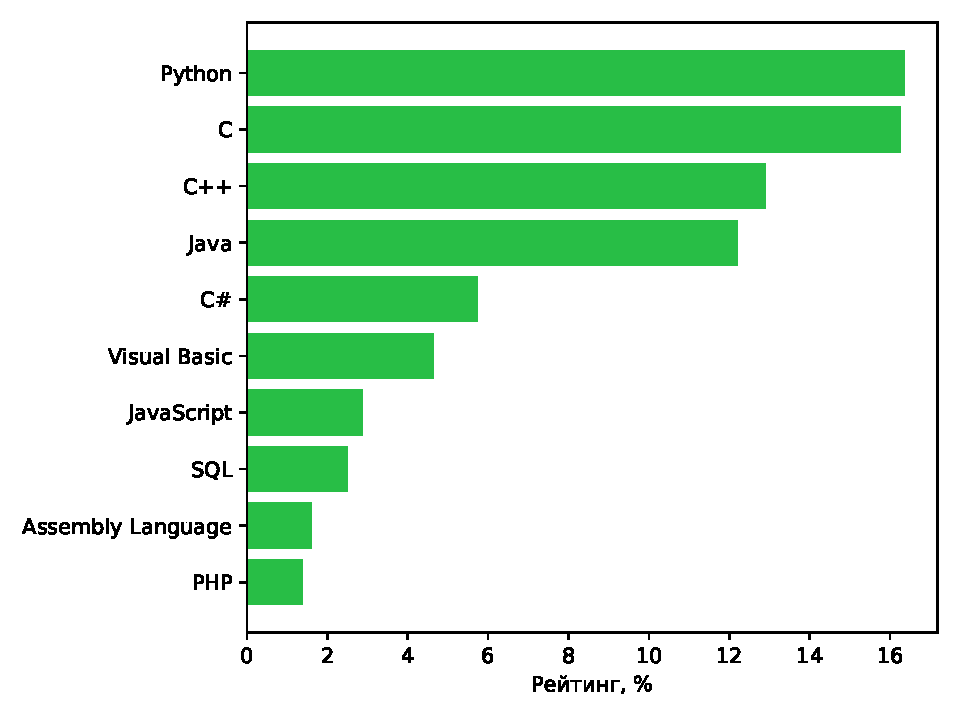
\includegraphics[width=\linewidth]{./pics/tiobe}
	\caption{Индекс \href{https://www.tiobe.com/tiobe-index/}{\textcolor{linkcolor}{TIOBE}} на январь 2023 года}
\end{figure}
\end{minipage}
\vfill
\end{frame}

\section{Простейшая программа на Python}

\begin{frame}[fragile]{Простейшая программа на Python}
\scriptsize
Простейшей программой на языке Python является пустой файл с расширением \texttt{.py}, однако рассмотрим традиционную реализацию программы, выводящей на экран сообщение <<Привет Мир!>>:

\begin{minted}{python}
|In [1]:| print('Привет Мир!')
|Привет Мир!|
\end{minted}

Для вывода на экран сообщения <<Привет Мир!>> достаточно обратиться к стандартной функции \mintinline{python}|print()| и передать ей в качестве параметра строку \texttt{'Привет Мир!'}.
\vfill
\end{frame}


\section{Имена идентификаторов}
\sectionframe

\begin{frame}[fragile]{Имена идентификаторов}
\scriptsize
\begin{itemize}
	\item \textcolor{extraorange}{\textbf{Переменные}}~-- это частный случай идентификаторов.
	\item \textcolor{extraorange}{\textbf{Идентификаторы}}~-- это имена, присвоенные чему-то для его обозначения.
\end{itemize}
\bigskip
При выборе имен идентификаторов необходимо соблюдать следующие правила:
\begin{enumerate}
	\item Первым символом идентификатора должна быть буква из алфавита (символ ASCII в верхнем или нижнем регистре, или символ Unicode), а также символ подчеркивания (<<\texttt{\_}>>);
	\item Остальная часть идентификатора может состоять из букв (символы ASCII в верхнем или нижнем регистре, а также символы Unicode), знаков подчеркивания <<\texttt{\_}>> или цифр ($0-9$);
	\item Имена идентификаторов \alert{\textbf{чувствительны}} к регистру!
\end{enumerate}
\bigskip
\alert{\textbf{Допустимые имена:}} \texttt{i}, \texttt{\_\_my\_name}, \texttt{name\_23}, \texttt{a1b2\_c3}

\alert{\textbf{{\color{red}Недопустимые имена:}}} \texttt{2things}, \texttt{my-name}, \texttt{>a1b2\_c3}
\vfill
\end{frame}

\begin{frame}[fragile]{Имена идентификаторов}
\scriptsize
\begin{itemize}
	\item Определяемые Вами имена не могут совпадать с \textbf{ключевыми словами} в Python.
	\item К примеру, если Вы попытаетесь выбрать для переменной имя \mintinline{ipython}|class|, то Python сообщит об ошибке.
\end{itemize}
\begin{table}[h!]
\caption{Ключевые слова в Python}
\centering
\begin{tabular}{p{0.15\linewidth}p{0.15\linewidth}p{0.15\linewidth}p{0.15\linewidth}p{0.15\linewidth}}
	
	\hline
	\mintinline{ipython}|False| & 
	\mintinline{ipython}|class| & \mintinline{ipython}|finally| & \mintinline{ipython}|is| &
	\mintinline{ipython}|return| \\
	
	\mintinline{ipython}|None| & 
	\mintinline{ipython}|continue| & \mintinline{ipython}|for| & \mintinline{ipython}|lambda| &
	\mintinline{ipython}|try| \\
	
	\mintinline{ipython}|True| & 
	\mintinline{ipython}|def| &
	\mintinline{ipython}|from| &
	\mintinline{ipython}|nonlocal| &
	\mintinline{ipython}|while| \\
	
	\mintinline{ipython}|and| & \mintinline{ipython}|del| &
	\mintinline{ipython}|global| &
	\mintinline{ipython}|not| &
	\mintinline{ipython}|with| \\
	
	\mintinline{ipython}|as| & \mintinline{ipython}|elif| &
	\mintinline{ipython}|if| &
	\mintinline{ipython}|or| &
	\mintinline{ipython}|yield| \\
	
	\mintinline{ipython}|assert| & \mintinline{ipython}|else| &
	\mintinline{ipython}|import| &
	\mintinline{ipython}|pass| &
	\mintinline{ipython}|break| \\
	
	\mintinline{ipython}|except| & \mintinline{ipython}|in| &
	\mintinline{ipython}|raise| &
	&
	\\ 
	\hline
\end{tabular}
\end{table}
\vfill
\end{frame}

\section{Динамическая типизация}
\sectionframe


\begin{frame}[fragile]{Динамическая типизация}
\scriptsize
\begin{itemize}
	\item Переменные никогда не располагают какой-либо информацией о типах или связанных с ними ограничениях.
	\item Понятие типа связано с объектами, а не именами.
	\item Переменные являются обобщенными по своей сути и просто ссылаются на определенные объекты в конкретный момент времени.

\begin{minted}{python}
|In [1]:| x = 1

|In [2]:| x = 'Hello'

|In [3]:| x = 1.2
\end{minted}
	\item Если переменная используется в каком-то выражении, то при его вычислении она заменяется объектом, ссылкой на который она является.
	\item Все переменные должны быть присвоены чему либо до того, как их можно будет использовать; использование неприсвоенных переменных приведет к ошибке!
\end{itemize}
\vfill
\end{frame}


\begin{frame}[fragile]{Ссылочная модель данных}
\scriptsize
В момент, когда происходит присваивание значений переменной:
\begin{minted}{python}
|In [1]:| a = 5
\end{minted}
фактически происходит выполнение трех шагов:

\begin{enumerate}
	\item Создание объекта для представления значения \texttt{5}.
	\item Создание переменной \mintinline{python}|a|.
	\item Связывание переменной \mintinline{python}|a| с новым объектом \texttt{5}.
\end{enumerate}

\centering
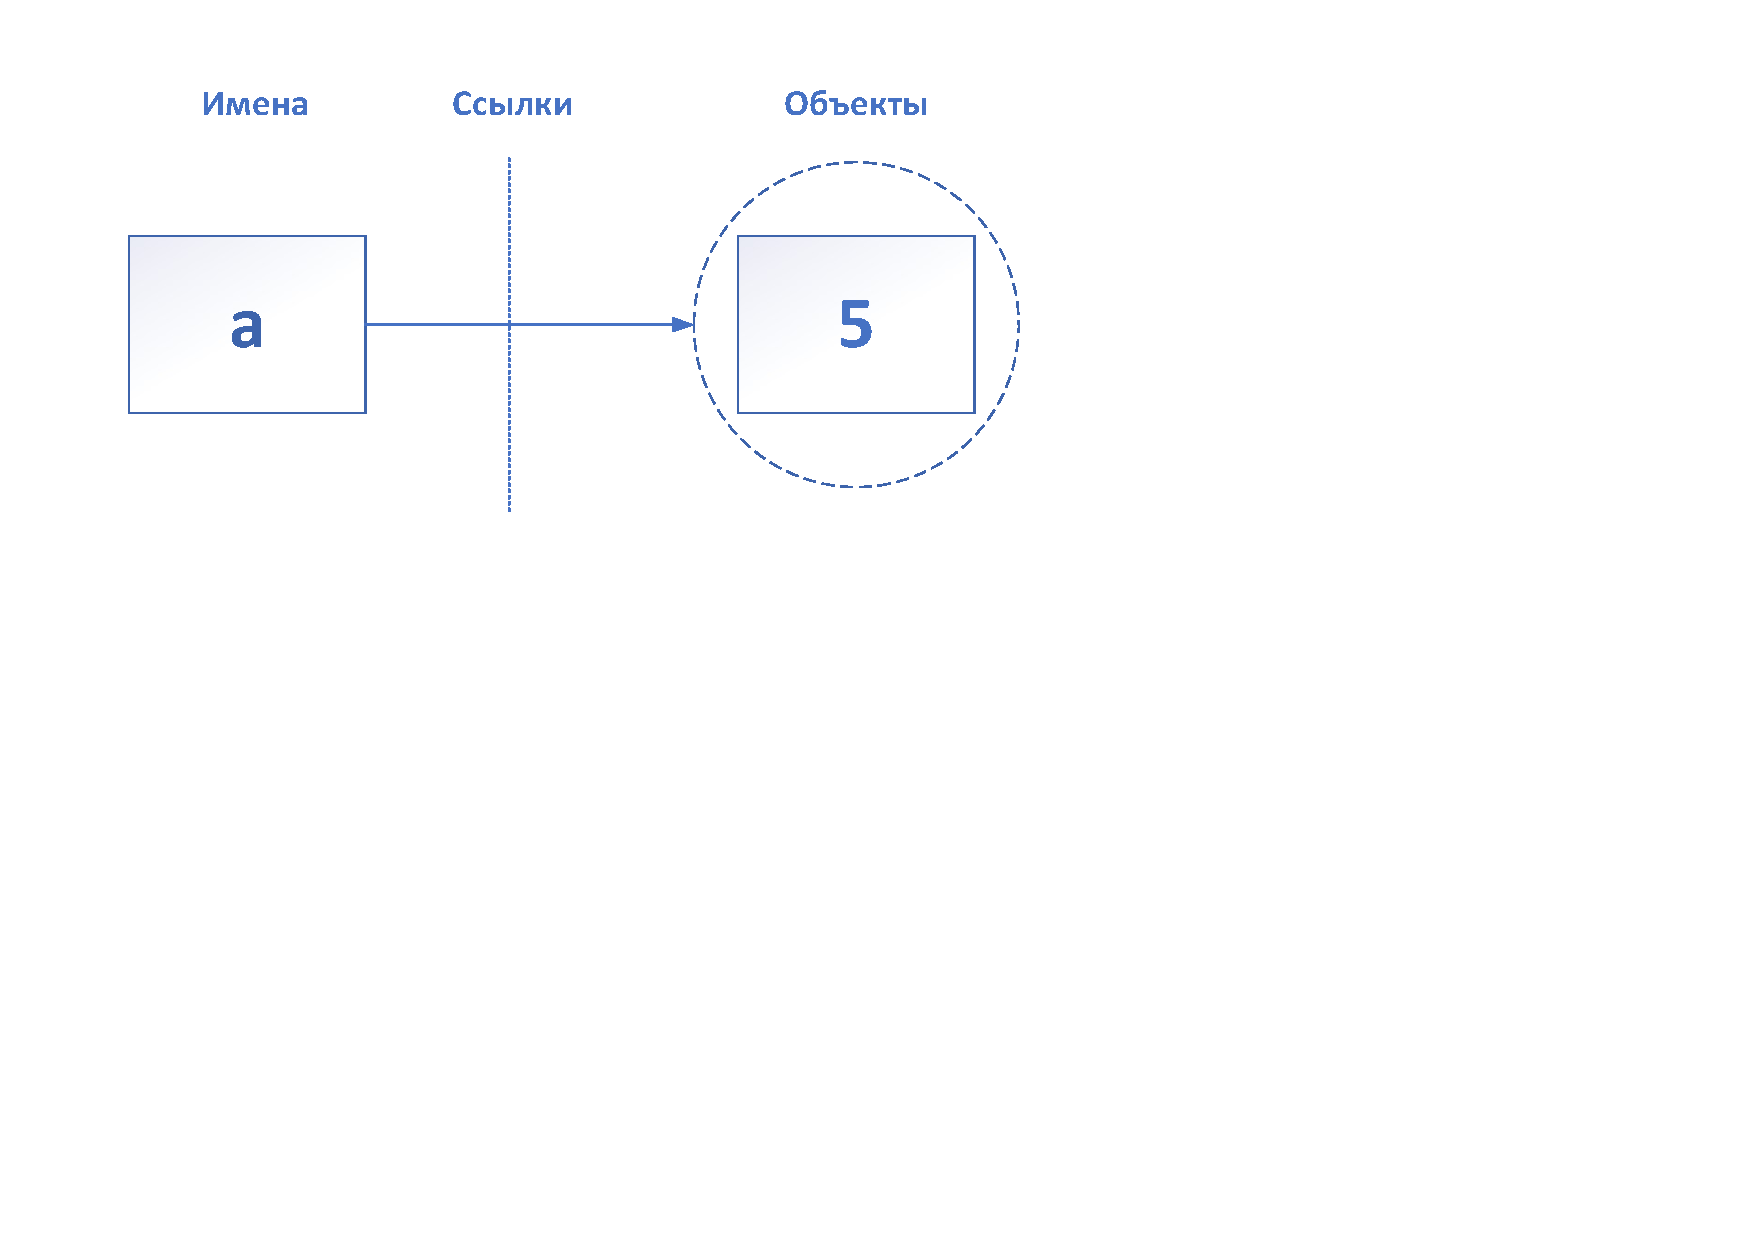
\includegraphics[width=.6\textwidth]{./pics/имена_и_объекты}

\vfill
\end{frame}


\begin{frame}[fragile]{Сборка мусора}
\scriptsize
В Python при присваивании имени нового объекта происходит освобождение области памяти, занимаемой предыдущим объектом, если на него не ссылается другое имя или объект. 

Данная операция известна как \alert{\textbf{сборка мусора}}:
\begin{minted}{python}
|In [1]:| x = 32 

|In [2]:| 'hello'  # Освободить память, занимаемую 32 (если нет других ссылок)

|In [3]:| x = 3.1245   # Освободить память, занимаемую 'hello'

|In [4]:| x = [0, 1, 2, 3] # Освободить память, занимаемую 3.1245
\end{minted}
\begin{itemize}
	\item Неоспоримое преимущество сборки мусора заключается в том, что она позволяет свободно использовать объекты без необходимости выделения и освобождения памяти вручную. 
	\item Python  будет автоматически выделять или очищать пространство для хранения объектов при выполнении программы.
\end{itemize}
\vfill	
\end{frame}

\section{Запись комментариев}
\sectionframe

\begin{frame}[fragile]{Запись комментариев}
\scriptsize
\textcolor{extraorange}{\textbf{Комментарии}}~-- это то, что пишется после \mintinline{python}|#| и представляет интерес лишь как заметка для читающего программу. Текст программы говорит о том, \textbf{как}, а комментарии должны объяснять, \textbf{почему}.
\begin{minted}{python}
|In [1]:| print('Привет Мир!')  # print - это функция 
\end{minted}
\begin{itemize}
	\item Комментарии могут встречаться в тексте программы как отдельные строки или могут быть размещены справа от операторов в строке.
	\item Текст после символов \mintinline{python}|#| пропускается интерпретатором как примечание, предназначенное для человека, читающего данную программу.
	\item При копировании кода Вы можете игнорировать комментарии, т.к. они носят   исключительно информативный характер.
	\item Грамотное использование комментариев может в значительной степени повысить читаемость, облегчить понимание и, как следствие, улучшить поддерживаемость Вашего программного кода.
\end{itemize}
\vfill
\end{frame}

\section{Типы данных}
\sectionframe


\begin{frame}[fragile]{Классификация объектов}
\scriptsize
Основные типы объектов в Python:
\begin{table}[h!]
\centering
\begin{tabular}{|p{0.325\textwidth}|p{0.325\textwidth}|p{0.3\textwidth}|}
	\hline
	\textbf{Тип объекта} & \textbf{Категория} & \textbf{Изменяемый?} \\
	\hline
	Числа (все) & Числовые & Нет \\	
	Строки & Последовательности & Нет \\	
	Списки & Последовательности & Да \\
	Словари & Отображения & Да \\
	Кортежи & Последовательности & Нет \\
	Файлы & Расширения & - \\
	Множества & Множества & Да \\
	\hline
\end{tabular}
\end{table}
\vfill
\end{frame}


\section{Числовые типы}
\sectionframe


\begin{frame}[fragile]{Числовые литералы}
\scriptsize
Числа в Python могут быть трех типов:
\begin{enumerate}
	\item Целые числа (\mintinline{ipython}|int|);
	\item Числа с плавающей точкой (\mintinline{ipython}|float|);
	\item Комплексные числа (\mintinline{ipython}|complex|).
\end{enumerate}
\begin{table}[h!] 
\centering
\begin{tabular}{|p{0.5\linewidth}|p{0.49\linewidth}|}
	\hline
	\textbf{Литерал} & \textbf{Расшифровка} \\
	\hline
	\mintinline{ipython}|1234|, \mintinline{ipython}|-24|, \mintinline{ipython}|0|, \mintinline{ipython}|99999999999999999| & Целые числа (неограниченный размер) \\
	\mintinline{ipython}|1.23|, \mintinline{ipython}|1.|, \mintinline{ipython}|3.17e-10|, \mintinline{ipython}|4E210|, \mintinline{ipython}|4.0e+210| & Числа с плавающей точкой \\
	\mintinline{ipython}|3+4j|, \mintinline{ipython}|3.0+4.0j|, \mintinline{ipython}|3J| & Литералы комплексных чисел \\
	\hline
\end{tabular}
\end{table}
\vfill
\end{frame}

\begin{frame}[fragile]{Целые числа и числа с плавающей точкой}
\scriptsize
\begin{itemize}
	\item Целые числа записываются в виде строк десятичных цифр. 
	\item Числа с плавающей точкой имеют десятичную точку и/или необязательный показатель степени со знаком, вводимый посредством нотации \texttt{e} или \texttt{E}.
	\item Целые числа можно создавать, используя встроенную функцию \mintinline{python}|int()|, а числа с плавающей точкой~-- при помощи встроенной функции \mintinline{python}|float()|:
\end{itemize}
\begin{minted}[fontsize=\tiny]{python}
|In [1]:| x = 2.5
   |...:| y = 1
   |...:| z = 2.

|In [4]:| type(x)  # Число с плавающей точкой
|float|

|In [5]:| type(y)  # Целое число
|int|

|In [6]:| type(z)  # Тоже число с плавающей точкой
|float|

|In [7]:| int(x)  # Получение целого числа отбрасыванием дробной части
|Out[7]: 2|

|In [8]:| float(y)  # Приведение целого числа к типу float
|Out[8]: 1.0|
\end{minted}
\vfill
\end{frame}

\section{Арифметические операции с числами}
\sectionframe	% section title is automatically capitalised

\begin{frame}[fragile]{Арифметические операции с числами}
\scriptsize
Основные арифметические операции с числами:
\begin{table}[h!]
\begin{tabular}{|p{0.15\linewidth}|p{0.2\linewidth}|p{0.6\linewidth}|}
	\hline
	\textbf{Приоритет} & \textbf{Операция} & \textbf{Описание} \\
	\hline
	4& \mintinline{ipython}|x + y| & Сложение \\
	4& \mintinline{ipython}|x - y| & Вычитание \\
	3& \mintinline{ipython}|x * y| & Умножение \\
	3& \mintinline{ipython}|x % y| & Остаток от деления (деление по модулю) \\
	3& \mintinline{ipython}|x / y|, \quad \mintinline{ipython}|x // y| & Настоящее деление, деление нацело (с округлением в меньшую сторону) \\
	2& \mintinline{ipython}|-x|, \quad \mintinline{ipython}|+x| & Противоположность, идентичность \\
	1& \mintinline{ipython}|x ** y| & Возведение в степень \\
	\hline
\end{tabular}
\end{table}
\begin{itemize}
	\item Если операция используется с двумя операндами, она называется \alert{\textbf{бинарной}}.
	\item Существуют также операции с одним операндом, называемые \alert{\textbf{унарными}}.
\end{itemize}
\vfill
\end{frame}


\begin{frame}[fragile]{Составные выражения}
\scriptsize
Подобно другим языкам программирования, сложные выражения в  Python записываются путем объединения арифметических операций. Например, определение суммы двух произведений можно представить в виде комбинации переменных и операций:
$$
a \cdot b + c \cdot d
$$

Значения подобных и еще более сложных выражений интерпретатор Python будет вычислять в соответствии с \alert{\textbf{приоритетом операций}}.

\bigskip
Заключение подвыражений в круглые скобки переопределяет приоритеты операций Python; выражения в круглых скобках во всех случаях вычисляются первыми и затем их результаты используются в охватывающих выражениях.
\begin{align*}
	(x &+ y) \cdot z \\
	x &+ (y \cdot z)
\end{align*}
\vfill
\end{frame}

\section{Некоторые математические функции}
\sectionframe

\begin{frame}[fragile]{Некоторые математические функции}
\scriptsize
\begin{itemize}
	\item В добавление к основным инструментам, Python также предлагает встроенные функции и стандартные модули для работы с числами.
	\item Например, встроенные функции \mintinline{python}|pow()| и \mintinline{python}|abs()| вычисляют степень и абсолютное значение, соответственно:
\end{itemize}
\begin{minted}[fontsize=\tiny]{python}
|In [1]:| import math

|In [2]:| math.pi, math.e                          # Общие константы
|Out[2]: (3.141592653589793, 2.718281828459045)|

|In [3]:| math.sin(2 * math.pi / 180)              # Синус
|Out[3]: 0.03489949670250097|

|In [4]:| math.sqrt(121), math.sqrt(3)             # Квадратный корень
|Out[4]: (11.0, 1.7320508075688772)|

|In [5]:| pow(3, 4), 3 ** 4, 3.0 ** 4.0            # Возведение в степень
|Out[5]: (81, 81, 81.0)|

|In [6]:| abs(-24.0), sum((1, 2, 3, 4, 5, ))       # Абсолютное значение, суммирование
|Out[6]: (24.0, 15)|

|In [7]:| min(3, 1, 2, 4, 5), max(3, 1, 2, 4, 5)   # Минимум, максимум
|Out[7]: (1, 5)|
\end{minted}
\vfill
\end{frame}

\begin{frame}[fragile]{Распространенные математические функции \\ модуля \texttt{math}}
\scriptsize
\begin{table}
\begin{tabular}{|p{.3\linewidth}|p{.69\linewidth}|}
	\hline
	\textbf{Литерал} & \textbf{Расшифровка} \\
	\hline
	\mintinline{ipython}|math.ceil(x)| & Округление до ближайшего большего числа \\
	\mintinline{ipython}|math.floor(x)| & Округление вниз \\
	\mintinline{ipython}|math.trunc(x)| & Усекает значение x до целого \\
	
	\mintinline{ipython}|math.exp(x)| & $e^x$ \\
	\mintinline{ipython}|math.log(x, [base])| & Логарифм \texttt{x} по основанию \texttt{base}; если \texttt{base} не указан, вычисляется натуральный логарифм. \\
	\mintinline{ipython}|math.acos(x)| & Арккосинус \texttt{x} в радианах \\
	\mintinline{ipython}|math.asin(x)| & Арксинус \texttt{x} в радианах \\
	\mintinline{ipython}|math.atan(x)| & Арктангенс \texttt{x} в радианах \\
	\mintinline{ipython}|math.cos(x)| & Косинус \texttt{x} (\texttt{x} указывается в радианах) \\
	\mintinline{ipython}|math.sin(x)| & Синус \texttt{x} (\texttt{x} указывается в радианах) \\
	\mintinline{ipython}|math.tan(x)| & Тангенс \texttt{x} (\texttt{x} указывается в радианах) \\
	\hline
\end{tabular}
\end{table}
\vfill
\end{frame}

\section{Пример}
\sectionframe

\begin{frame}[fragile]{Пример}
\footnotesize
Вычислить y:
\begin{Large}
\begin{equation*}
	y = \dfrac{a + 2 \cdot b ^ 3}{\dfrac{a}{x} + \left(x + a\right)^3} + \dfrac{\left(\sin\left(k\right)\right)^2}{\ln \left(k + m\right)}
\end{equation*}
\end{Large}

\begin{center}
$a = 2.6e3$; \quad $x = 3.18$; \quad $m = 25$; \quad $b = 1.4$; \quad $k = 4$.
\end{center}
\vfill
\end{frame}

\begin{frame}[fragile]{Пример}
\scriptsize
\begin{equation*}
	y = \dfrac{a + 2 \cdot b ^ 3}{\dfrac{a}{x} + \left(x + a\right)^3} + \dfrac{\left(\sin\left(k\right)\right)^2}{\ln \left(k + m\right)}
\end{equation*}
\begin{center}
	$a = 2.6e3$; \quad $x = 3.18$; \quad $m = 25$; \quad $b = 1.4$; \quad $k = 4$.
\end{center}
\begin{minted}[fontsize=\tiny]{python}
|In [1]:| import math

|In [2]:| a = 2.6e3
   |...:| x = 3.18
   |...:| m = 25
   |...:| b = 1.4
   |...:| k = 4

|In [3]:| y = (a + 2 * b ** 3) / (a / x + (x + a) ** 3) + math.sin(k) ** 2 / math.log(k + m)
   |...:| y
|Out[3]: 0.17009212827361847|
\end{minted}
\vfill
\end{frame}

\section{Задание}
\sectionframe


\begin{frame}[fragile]{Задание}
\footnotesize	
Вычислите выражения при $x = 3$:
\begin{enumerate}
	\item $y = \sqrt[5]{\left(x + 2\right)^4 + \sin \left(x\right)} + \sqrt{\log _{10}\left(x + \dfrac{x^2}{2}\right)} + 5.8 \cdot 10^{-7} \cdot x$
	
	\item $y = \dfrac{\sqrt{x^2 + \sin \left(\dfrac{1}{4 \cdot x}\right)}}{\ln \left(3 \cdot x\right) + x} + 4 \cdot 10^{-5}$
	
	\item $y = 7.2 \cdot 10^{-4} \cdot \dfrac{\sqrt{\left|1 - \left(\sin \left(x\right)\right)^2\right|}}{e^{-{4}/{x}}}$
	
	\item $y = \dfrac{1 - 2 \cdot x \cdot \sin \left(x\right)}{\ln \left(\dfrac{5}{x}\right)} + e^{x^2}$
	
	\item $y = \dfrac{\sin \left(x^2\right)}{e^{{x}/{2}} \cdot \ln \left(x + 1\right)} + 2.3 \cdot 10^{-7}$
	
\end{enumerate}

\vfill
\end{frame}

\begin{frame}[fragile]{Задание}
\footnotesize	
\begin{enumerate}
	\setcounter{enumi}{5}
	
	\item $y = \dfrac{\dfrac{x}{\sin \left(x\right) + 1}}{\dfrac{e^{x^2} + \ln \left(x\right)}{\sqrt{x^2 + 3.7 \cdot 10 ^{-5} \cdot x}}}$
	
	\item $y = \dfrac{4.9 \cdot 10^{-2} + \ln \left(\dfrac{x^2}{2}\right)}{\arctan \left(x^2 + 2 \cdot x\right)}$
\end{enumerate}

\vfill
\end{frame}

\contactsframe[\Large \textbf{Благодарю за внимание!}]{
	
	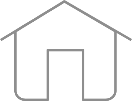
\includegraphics[width=.05\textwidth]{pics/home} \quad Учебный корпус №2, ауд. 136 \\
	
\includegraphics[width=.05\textwidth]{pics/mail} \quad chuva@tpu.ru \\
	
\includegraphics[width=.03\textwidth]{pics/tel} \quad +7-962-782-66-15
}

\end{document}

